\documentclass[a4paper,11pt]{extarticle} % тип документа
\usepackage[left=1.6cm,right=1.6cm, margin=2cm]{geometry}
%%%Библиотеки
    %\usepackage[warn]{mathtext}	
    \usepackage[T2A]{fontenc}   %Кодировка
\usepackage[utf8]{inputenc} %Кодировка исходного текста
\usepackage{enumitem}
    \usepackage[english, russian]{babel} %Локализация и переносы
    \usepackage{caption}
    \usepackage{listings}
    \usepackage{amsmath, amsfonts, amssymb, amsthm, mathtools}
    \usepackage[warn]{mathtext}
    \usepackage[mathscr]{eucal}
    \usepackage{wasysym}
    \usepackage{graphicx} %Вставка картинок правильная
    \usepackage{indentfirst}
    \usepackage{float}    %Плавающие картинки
    \usepackage{wrapfig}  %Обтекание фигур (таблиц, картинок и прочего)
    \usepackage{fancyhdr} %Загрузим пакет
    \usepackage{lscape}
    \usepackage{xcolor}
    \usepackage[normalem]{ulem}
    
    \usepackage{titlesec}
    \titlelabel{\thetitle.\quad}

\title{Лабораторная работа № 4.3.1 \\ Изучение дифракции света}
\date{}
\author{Котова Александра, Чекмарёв Игорь}
\begin{document}

\maketitle

\section{Теоретические сведения}
\subsection{Введение} Дифракция --- волновое явление, проявляющееся в отклонении от прямолинейного распространения света по законам геометрической оптики, если если оно не может быть истолковано как результат отражения, преломления или изгибания световых лучей в средах с непрерывно меняющимся показателем преломления. В основе описания дифракции лежит \textit{принцип Гюйгенса--Френеля}: каждый элемент волнового фронта можно рассматривать как источник вторичных сферических волн, а результирующее световое поле в точке наблюдения определяется интерференцией этих волн. 


В основе описания дифракции лежит принцип Гюйгенса-Френеля, который заключается в том, что каждый
элемент волнового фронта является центром возмущения, порождающего вторичные сферические волны,
в результате интерференции которых формируется результирующее световое поле в каждой точке
пространства. Схема, поясняющая принцип Гюйгенса-Френеля, изображена на рис. 1.


\begin{figure}[H]
		\center{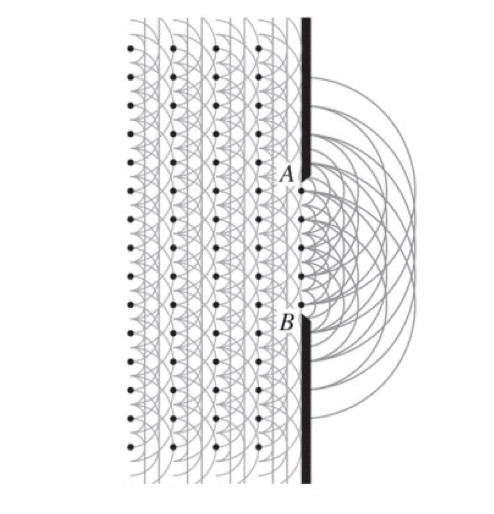
\includegraphics[scale=0.63]{gu_fr.png}}
		\caption{Иллюстрация принципа Гюйгенса-Френеля при дифракции на щели. Плоская волна при распространении
в каждой плоскости даёт набор точечных источников сферических волн. При попадании на препятствие волны
вторичные точечные источники дают интерферирующие волны, которые складываются в дифракционную картину.}
	\end{figure}

\subsection{Дифракция Френеля и распределение интенсивности волнового поля в центре за круглым отверстием}
Рассмотрим бесконечный транспарант, в котором сделано круглое отверстие радиусом $r$. На это
отверстие падает плоская волна с длиной $\lambda$ а за ним на расстоянии $z$ расположен экран, на котором
ведётся наблюдение результирующей картины. Нас будет интересовать расчёт интенсивности в точке $P$
лежащей на оси симметрии системы (см. рис. 2).


\begin{figure}[H]
		\center{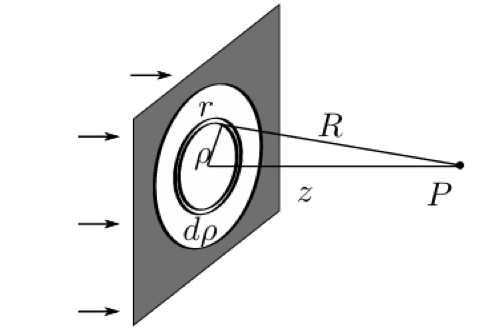
\includegraphics[scale=0.73]{raspr_intents.png}}
		\caption{Схема к постановке задачи о дифракции Френеля на круглом отверстии. Транспарант представляет собой
бесконечный поглощающий экран с круговым отверстием радиуса $r$ на оси симметрии системы на расстоянии $z$
находится точка $P$ наблюдения.}
	\end{figure}


Для применения принципа Гюйгенса-Френеля разобьем открытую часть волнового фронта (поверхность,
совпадающую с плоскостью отверстия) на узкие концентрические кольцевые зоны — \textit{зоны Френеля}.
Границы зон проводятся так, чтобы расстояние от края каждой зоны до точки $P$ отличалось ровно на $\lambda/2$
(т.е. расстояние от точки наблюдения $P$ до точек кольца \textit{$z + m\lambda/2$}, где $m$ – целое число). Это означает,
что вторичные волны от соседних зон приходят в точку в противофазе. Исходя из такого определения, мы
можем записать для $m$-ой зоны Френеля разность хода по отношению к центральному источнику:


\begin{equation}
\Delta_m = \sqrt{z^2 + r_m^2} - z \approx \frac{r_m^2}{2z} = \frac{m\lambda}{2},
\end{equation}

откуда радиус $m$-й зоны Френеля равен

\begin{equation}
r_m = \sqrt{m\lambda z}.
\end{equation}

Вклады соседних зон приходят в точку наблюдения практически в противофазе, поэтому суммирование амплитуд удобно представлять векторной диаграммой. Такая диаграмма приводит к спирали Френеля.

Характерное свойство спирали Френеля заключается в том, что, когда открыто нечетное число зон, конец
вектора оказывается в верхней части спирали (далеко от первого вектора), что даёт максимум
интенсивности. Когда открыто четное число зон — в нижней части (близко к первому вектору), что дает
минимум.

\begin{figure}[H]
		\center{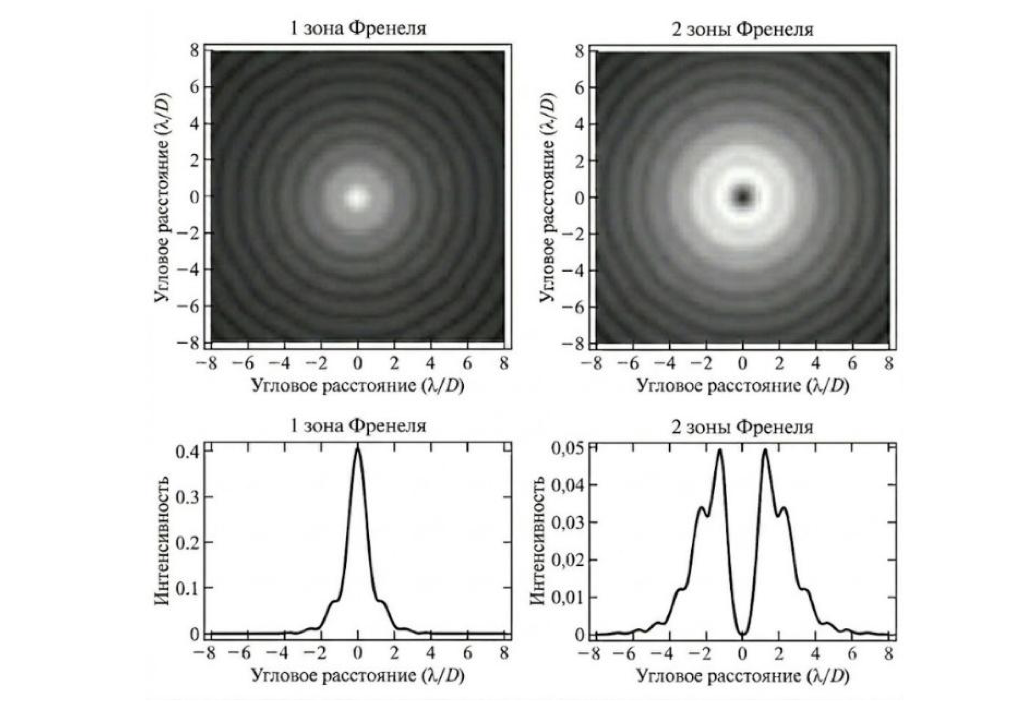
\includegraphics[scale=0.73]{hernya.png}}
		\caption{результат распределения интенсивности в плоскости наблюдения. Центр наблюдения отвечает точке $P$. $D$ –
диаметр открытого отверстия}
	\end{figure}

Удобно ввести число открытых зон Френеля
$N = \frac{r^2}{\lambda z}$, либо волновой параметр $p = \frac{\sqrt{\lambda z}}{r} = \frac{1}{N^2}$

Тогда можно выделить три режима:
\begin{enumerate}[label=\arabic*)]
    \item предел геометрической оптики: $p \ll 1$;
    \item дифракция Френеля(в ближней волновой зоне): $p \sim 1$;
    \item дифракция Фраунгофера(в дальней волновой зоне, или в параллельных лучах): $p \gg 1$.
\end{enumerate}


\subsection{Дифракция Фраунгофера на круглом отверстии}

При дифракции плоской волны на круглом отверстии в непрозрачном экране на удалённой плоскости
наблюдения (при условии $p \gg 1$) образуется картина дифракции, показанная на Рис.4 : центральное
яркое дифракционное пятно (которое называется пятном Эйри) окружено чередующимися светлыми и
тёмными кольцами. Угловая полуширина пятна Эйри (главного максимума в
картине $I(\theta)$ определяется условием

\begin{equation}
\sin\theta = 0.61\,\frac{\lambda}{r}.
\end{equation}

\begin{figure}[H]
		\center{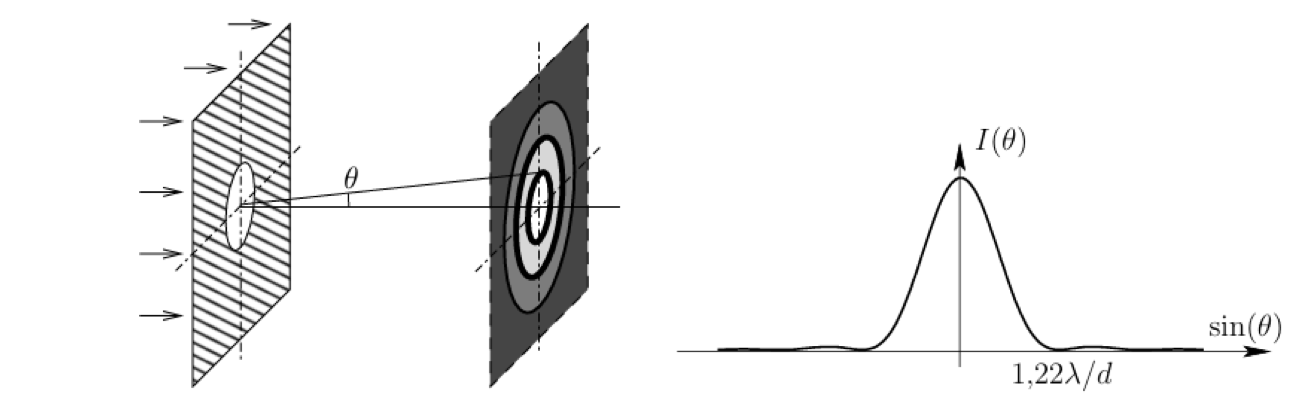
\includegraphics[scale=0.73]{another_bullshit.png}}
		\caption{Слева - геометрия задачи дифракции Фраунгофера на круглом отверстии. Справа - угловое распределение интенсивности в центральном сечении. Дифракционная картина сосредоточена в основном в главном дифракционном максимуме.}
	\end{figure}



% Для круглого непрозрачного препятствия используется принцип Бабине: сумма амплитуд полей, получаемых от двух взаимно дополнительных экранов, равна амплитуде поля при отсутствии экрана. Это позволяет свести задачу дифракции на непрозрачном диске к задаче дифракции на отверстии той же формы и, в частности, объяснить наличие пятна Пуассона в центре тени.




\subsection{Дифракция Френеля на щели}

Рассмотрим дифракцию плоской волны на щели, считая заданной её ширину $b$, а длину – бесконечной для
одномерности задачи. Пусть точка наблюдения $P$ расположена на расстоянии $z$ от щели.

\begin{figure}[H]
		\center{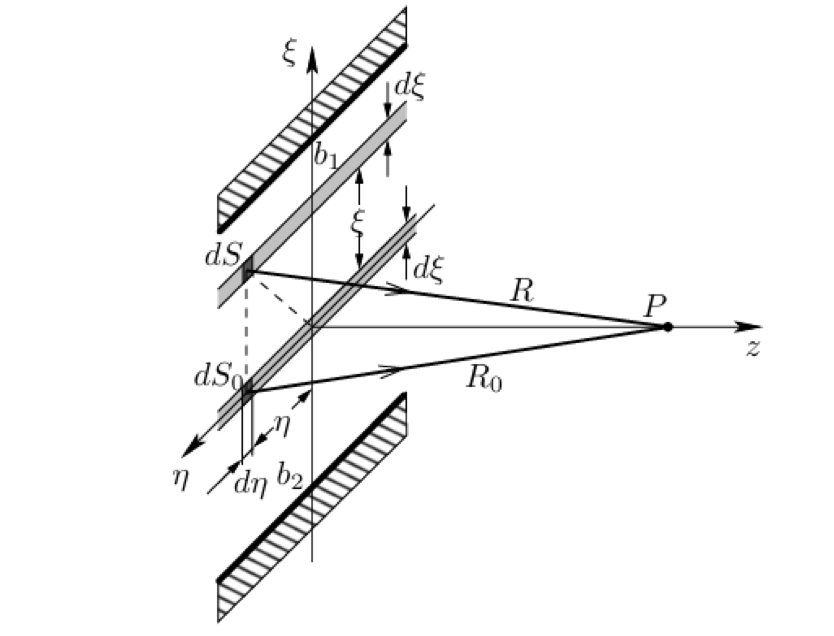
\includegraphics[scale=0.43]{more_bullshit.png}}
		\caption{Схема к постановке задачи о дифракции Френеля на щели. Транспарант представляет собой бесконечный поглощающий экран с горизонтальной щелью ширины $b$}
	\end{figure}


Разобьём щель на узкие полоски ширины $d\xi$, параллельные её краям. Разность фаз между соседними полосками равна

$$
d\varphi = k\left(\sqrt{z^2 + (\xi + d\xi)^2} - \sqrt{z^2 + \xi^2}\right)
\approx k\frac{\xi\,d\xi}{z},
$$

где $k = 2\pi/\lambda$. В данном случае вместо кольцевых зон Френеля, отвечающим колебаниям с набором фазы $\pi$
получаются зоны в виде полос (их называют \textit{зонами Шустера}) на расстояниях 
\begin{equation}
\xi_m = \sqrt{m\lambda z}.
\end{equation}
от точки наблюдения $P$.

В результате наблюдений дифракции Френеля на щели можно сопоставить распределение интенсивности
в соответствующей точке: 

\begin{figure}[H]
		\center{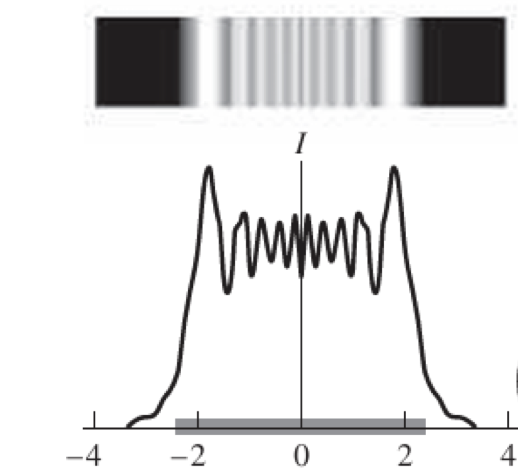
\includegraphics[scale=0.53]{greater_bullshit.png}}
		\caption{Сверху - пример дифракционной френелевской картины на щели. Снизу - распределение интенсивности по ширине щели}
	\end{figure}
\subsection{Дифракция Фраунгофера на щели}
Дифракция Фраунгофера (дифракция в дальней волновой зоне, или дифракция в параллельных лучах)
наблюдается в случае большого волнового параметра, что при заданных геометрических параметрах
препятствия она наблюдается на больших расстояниях. Оценим дальность для щели шириной $b$ = 1 мм и 
$\lambda$ = 500 нм: $z =
b^2/\lambda = 2 $ м. Для локализации этой картины используют дополнительную линзу за 
препятствием, фокусирующие параллельные лучи в соответствующие точки в фокальной плоскости.
На Рис.7 изображена типичная схема по наблюдению дифракции Фраунгофера на щели.

\begin{figure}[H]
		\center{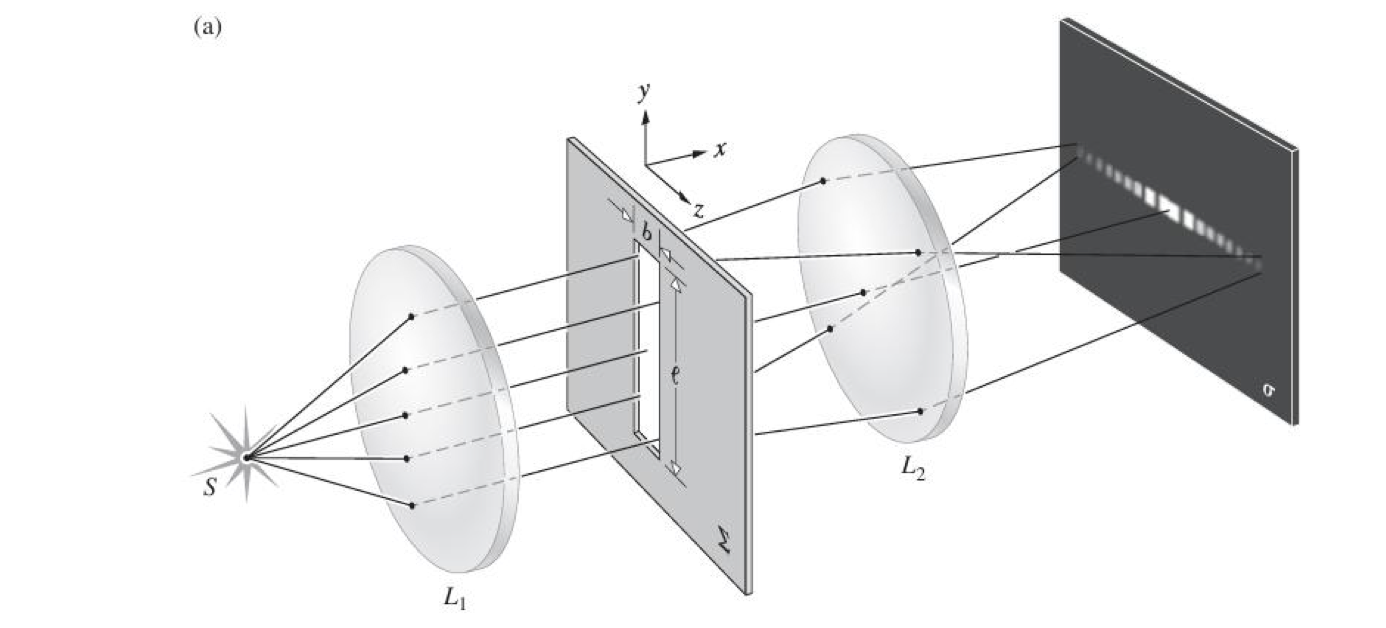
\includegraphics[scale=0.43]{very_bullshit.png}}
		\caption{Типичная схема для наблюдения дифракции Фраунгофера на щели. Тонкая линза $L_1$ преобразует волновой
фронт от источника $S$ в плоский для освещения щели, находящейся в плоскости транспаранта $\Sigma$. Прошедшее
излучение фокусируется линзой $L_2$ на экран.}
	\end{figure}

\begin{figure}[H]
		\center{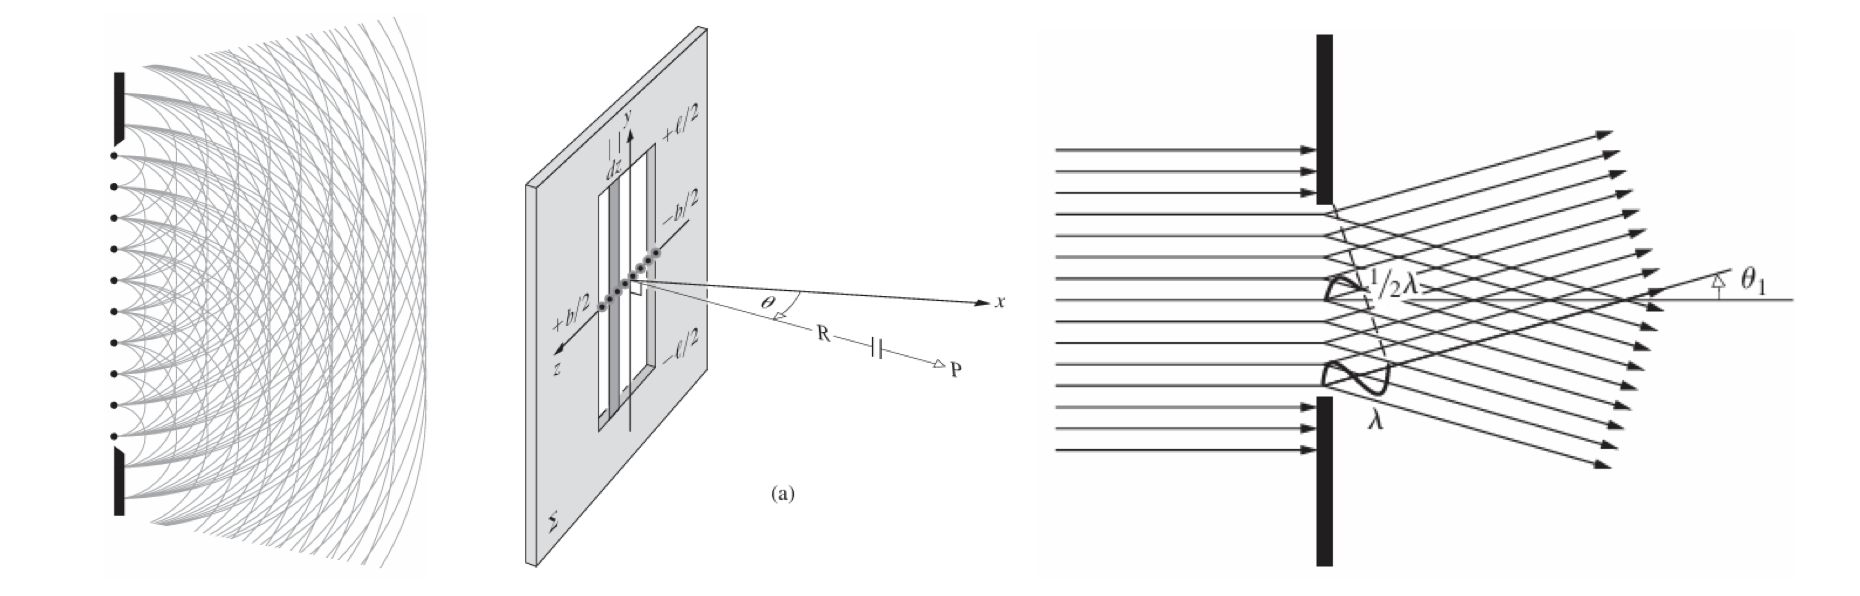
\includegraphics[scale=0.43]{badass_bullshit.png}}
		\caption{Представление волны в плоскости щели и за ней в виде суперпозиции волн от точечных источников}
	\end{figure}




Пусть щель разбита на $N$ одинаковых элементарных источников, находящихся на расстоянии $d$ друг от друга, так что $b = Nd$. Тогда разность фаз между соседними источниками равна

\begin{equation}
\alpha = kd\sin\theta.
\end{equation}

Суммарная амплитуда поля оказывается пропорциональной

\begin{equation}
E(\theta) \propto \frac{\sin(N\alpha/2)}{\sin(\alpha/2)}.
\end{equation}

В пределе $N \gg 1$ для интенсивности получаем классическую формулу дифракции Фраунгофера на щели:

\begin{equation}
I(\theta) = I(0)\left(\frac{\sin\beta}{\beta}\right)^2,
\qquad
\beta = \frac{\pi b\sin\theta}{\lambda}.
\end{equation}

Минимумы интенсивности(темные полосы) определяются условием

\begin{equation}
b\sin\theta_n = n\lambda,
\qquad n = \pm 1, \pm 2, \ldots
\end{equation}

а в фокальной плоскости линзы с фокусным расстоянием $f$ их координаты равны

\begin{equation}
x_n = f\tan\theta_n \approx \frac{fn\lambda}{b}.
\end{equation}


\subsection{Дифракция Фраунгофера на двух щелях}

Для двух одинаковых щелей ширины $b$, расстояние между которыми равно $d$, распределение интенсивности представляет собой интерференционные полосы, модулированные дифракционной огибающей:

\begin{equation}
I(\theta) = I(0)\left(\frac{\sin\beta}{\beta}\right)^2 \bigl(1 + \cos(kd\sin\theta)\bigr).
\end{equation}

Положения интерференционных максимумов определяются соотношением

\begin{equation}
d\sin\theta_m = m\lambda,
\qquad m = 0, \pm 1, \pm 2, \ldots
\end{equation}


а расстояние между соседними интерференционными полосами в фокальной плоскости линзы равно

\begin{equation}
\delta x = \frac{f\lambda}{d}.
\end{equation}


Поскольку полная угловая ширина главного дифракционного максимума (от минимума до минимума)
равна $2 \lambda / b$, где $b$ — ширина отдельной щели, то на нём укладывается $N = 2d/b$ тёмных
интерференционных полос (в центре картины максимум, поэтому светлых полос — на одну больше).

\begin{figure}[H]
		\center{
\includegraphics[scale=0.53]{comprehensive_bullshit .png}}
		\caption{Слева - картины дифракции на одной щели (сверху) и на двух одинаковых щелях той же ширины(снизу). Справа - распределение
интенсивности за двойной щелью.}
	\end{figure}




Для наблюдения чёткой интерференционной картины необходимо, чтобы расстояние между щелями не превышало радиус когерентности источника:

\begin{equation}
d \leq \rho_{\text{ког}} \approx \frac{\lambda f_1}{a},
\end{equation}

где $a$ --- размер протяжённого источника света, а $f_1$ --- фокусное расстояние линзы, формирующей плоскую волну.

\section{{Ход работы}}

\subsection{Дифракция Френеля на щели}
\begin{figure}[H]
		\center{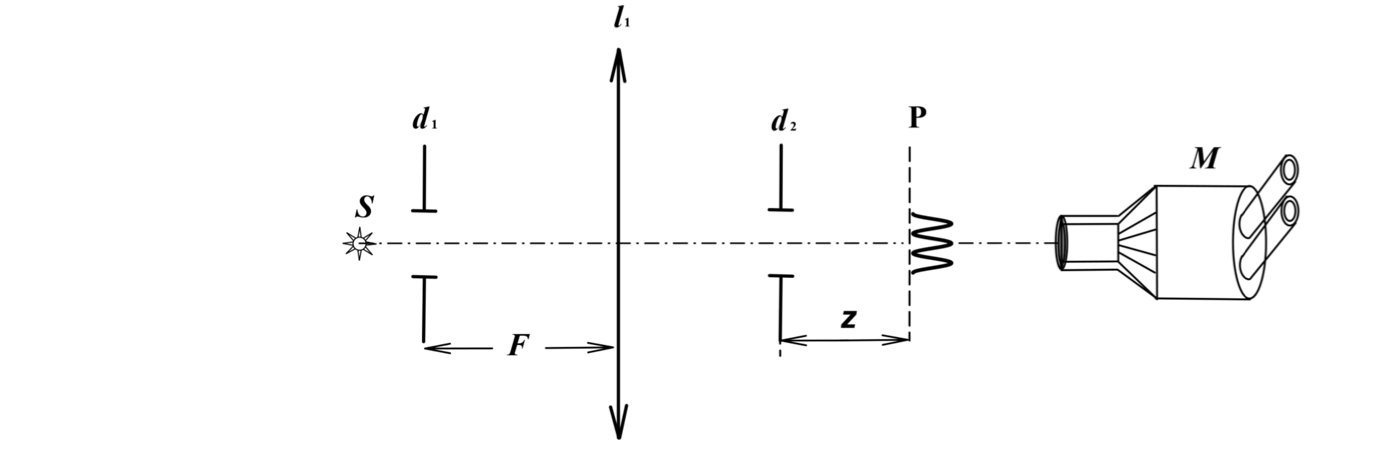
\includegraphics[scale=0.53]{urgent_bullshit.png}}
		\caption{Схема установки для наблюдения дифракции Френеля}
	\end{figure}
Для наблюдения дифракции Френеля соберем оптическую схему согласно
рис. 1. На оптической скамье следует последовательно установить и отцентрировать источник света S, оптическую щель $d_1$, которая играет роль вторичного
источника света, линзу $l_1$, вторую оптическую щель $d_2$ и микроскоп $M$. У источника света, зеленого лазера, $\lambda = 515 \text{ нм}$.

\par 

Щель $d_1$ вводится в установку с целью формирования условий, необходимых для наблюдения дифракции Френеля. Её назначение можно описать следующим образом: 
\begin{enumerate}[label=\arabic*)]
    \item  Формирование квазиточечного источника.
   Протяжённый источник света (S) заменяется узкой щелью $d_1$, которая ограничивает его поперечные размеры. В результате излучение, падающее на щель $d_2$, можно рассматривать как исходящее из квазиточечного источника.

\item Обеспечение пространственной когерентности.
   Сужение пучка с помощью щели $d_1$ уменьшает угловой размер источника, вследствие чего увеличивается пространственная когерентность излучения. Это является необходимым условием для наблюдения устойчивой дифракционной картины.

\item Формирование сферической волны.
   После прохождения через щель $d_1$ световая волна приобретает вид расходящейся сферической волны, что соответствует условиям дифракции Френеля - дифракции в ближней волновой зоне.

\end{enumerate}

Таким образом, щель $d_1$ необходима для преобразования излучения протяжённого источника в квазимонохроматическую, пространственно когерентную сферическую волну.



Значения микрометрического винта будем сразу пересчитывать в размер ширины щели, учитывая аппроксимирующую функцию $d(x) = 1.817829 \cdot 10^{-8}
\cdot x^2 - 4.641328 \cdot 10^{-4} \cdot x + 1.662572$.
Здесь ширина щели $[d(x)] = [\text{мм}]$, $x$ - показания микрометрического винта в мкм.



Цена деления микрометрического винта составляет $c = 0.05\ \text{мм} = 50\ \text{мкм}.$


Инструментальная погрешность отсчёта принимается равной половине цены деления: $
\Delta x = \frac{c}{2} = 25\ \text{мкм}.$

Погрешность ширины щели определяется по формуле распространения погрешности:
\begin{equation}
\Delta d \approx \left| \frac{d(d)}{dx} \right|\Delta x.
\end{equation}

Найдём производную:
\begin{equation}
\frac{d(d)}{dx} = 3.635658\cdot 10^{-8}x - 4.641328\cdot 10^{-4}.
\end{equation}

Тогда
\begin{equation}
\Delta d \approx \left|3.635658\cdot 10^{-8}x - 4.641328\cdot 10^{-4}\right|\cdot 25.
\end{equation}

При $x = 3400\ \text{мкм}$:
\begin{equation}
d'(3400) \approx -3.405 \cdot 10^{-4},
\end{equation}
\begin{equation}
\Delta d \approx 3.405 \cdot 10^{-4} \cdot 25 \approx 0.0085\ \text{мм}.
\end{equation}

Таким образом, инструментальная погрешность определения ширины щели составляет
\begin{equation}
\Delta d \approx 0.01\ \text{мм}.
\end{equation}


Определим начальное положение микроскопа, положение нуля - координату по шкале продольной линейки,
расположенной на оптической скамье, а также ширину щели $d_2$ за счет показаний микрометрического винта на ней:

$$
b^\text{винт} = (0.30 \pm 0.01)  \text{ мм;  }  x_0 = (101.0 \pm 0.5)\text{ cм}
$$

Приближая микроскоп $M$ к щели $d_2$, измерим зависимость координаты
микроскопа $z = x_0 - x_n$ от числа $n$ наблюдаемых тёмных полос, приняв $\sigma_z = 0.5$ см: 

% \begin{table}[H]
% \centering
% \begin{tabular}{|c|c|c|}
% \hline
% n & $x_n$, см & $z$, см\\
% \hline
% 1 & 96 & 5 \\
% \hline
% 2 & 97.5 & 3.5 \\
% \hline
% 3 & 98.8 & 2.2 \\
% \hline
% 4 & 99.2 & 1.8 \\
% \hline
% 5 & 99.7 & 1.3 \\
% \hline
% \end{tabular}

% \end{table}


\begin{table}[H]
\centering
\begin{tabular}{|c|c|c|c|c|}
\hline
\text{n} & $x_n$, см & \text{z, см} & $\sqrt{1/n}$ & $\sqrt{z}$, $\sqrt{\text{см}}$ \\
\hline
1 & 96 & 5 & 1 & 2.24 \\
\hline
2 & 97.5 & 3.5 & 0.707 & 1.77 \\
\hline
3 & 98.8 & 2.2 & 0.577 & 1.48 \\
\hline
4 & 99.2 & 1.8 & 0.5 & 1.34 \\
\hline
5 & 99.7 & 1.3 & 0.447 & 1.14 \\
\hline
\end{tabular}
\caption{Зависимость координаты микроскопа $z$ от числа $ n $ тёмных полос}
\end{table}


Построим график зависимости $z(n)$ в координатах $\sqrt{z}(1/\sqrt{n})$, чтобы провести линейную аппроксимацию:

\begin{figure}[H]
		\center{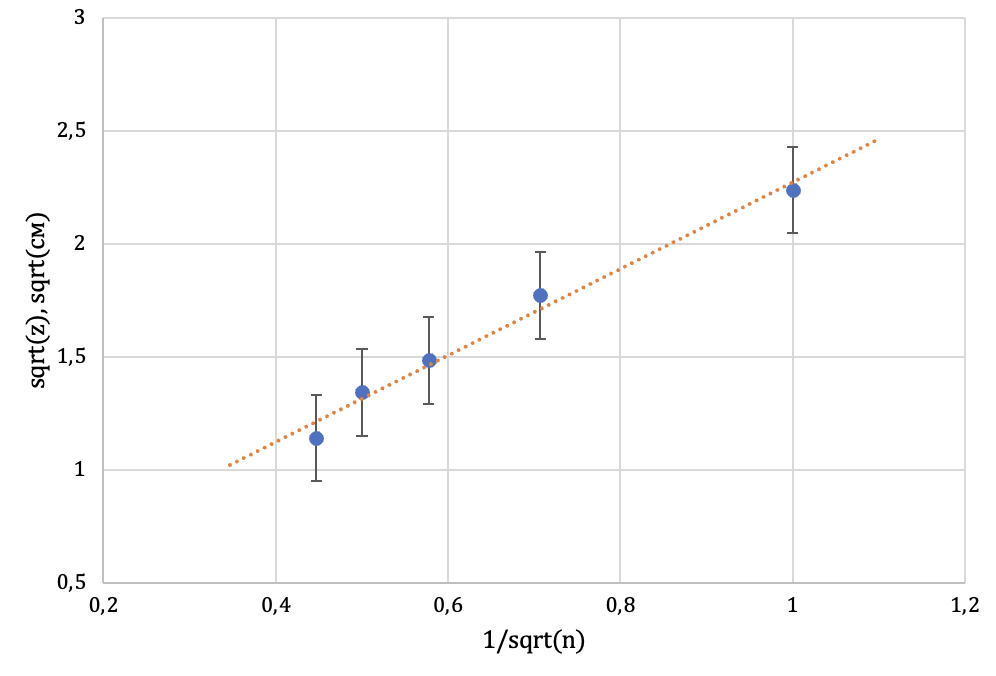
\includegraphics[scale=0.63]{hazard_bullshit.png}}
		\caption{график зависимости $\sqrt{z}(1/\sqrt{n})$}
	\end{figure}

Определим коэффицент наклона прямой по МНК: 
$$k = 1.91 \pm 0.15$$
Та погрешность, которую мы получили из МНК - это полученная оценка стандартного отклонения. Но это верно строго при «бесконечном числе данных», а точек в данном измерении всего 5. Погрешность коэффициента наклона, полученная методом наименьших квадратов, может быть скорректирована с учётом малого числа измерений с использованием коэффициента Стьюдента:
\[
\Delta k = t_{P,\nu}\, s_k
\]
где $s_k$ - ошибка из МНК, $\nu = N - 2$, где $N$ - число точек, $P$ - доверительная вероятность, уровень уверенности, с которым  хотим утверждать результат. Возьмем $P = 0.95$, $\nu = 5 - 2 = 3$.
\[
\Delta k = t_{P,\nu}\, s_k = 3.18 \cdot s_k \approx 0.47
\]

Тогда из формулы (4) можно получить $b = 2k\cdot \sqrt{\lambda} = (0.27 \pm 0.06)$ мм. 

Определим также размер щели по экрану монитора: 
установим, что 1 мм равен 894 пикселям (Рис.12):
\begin{figure}[H]
		\center{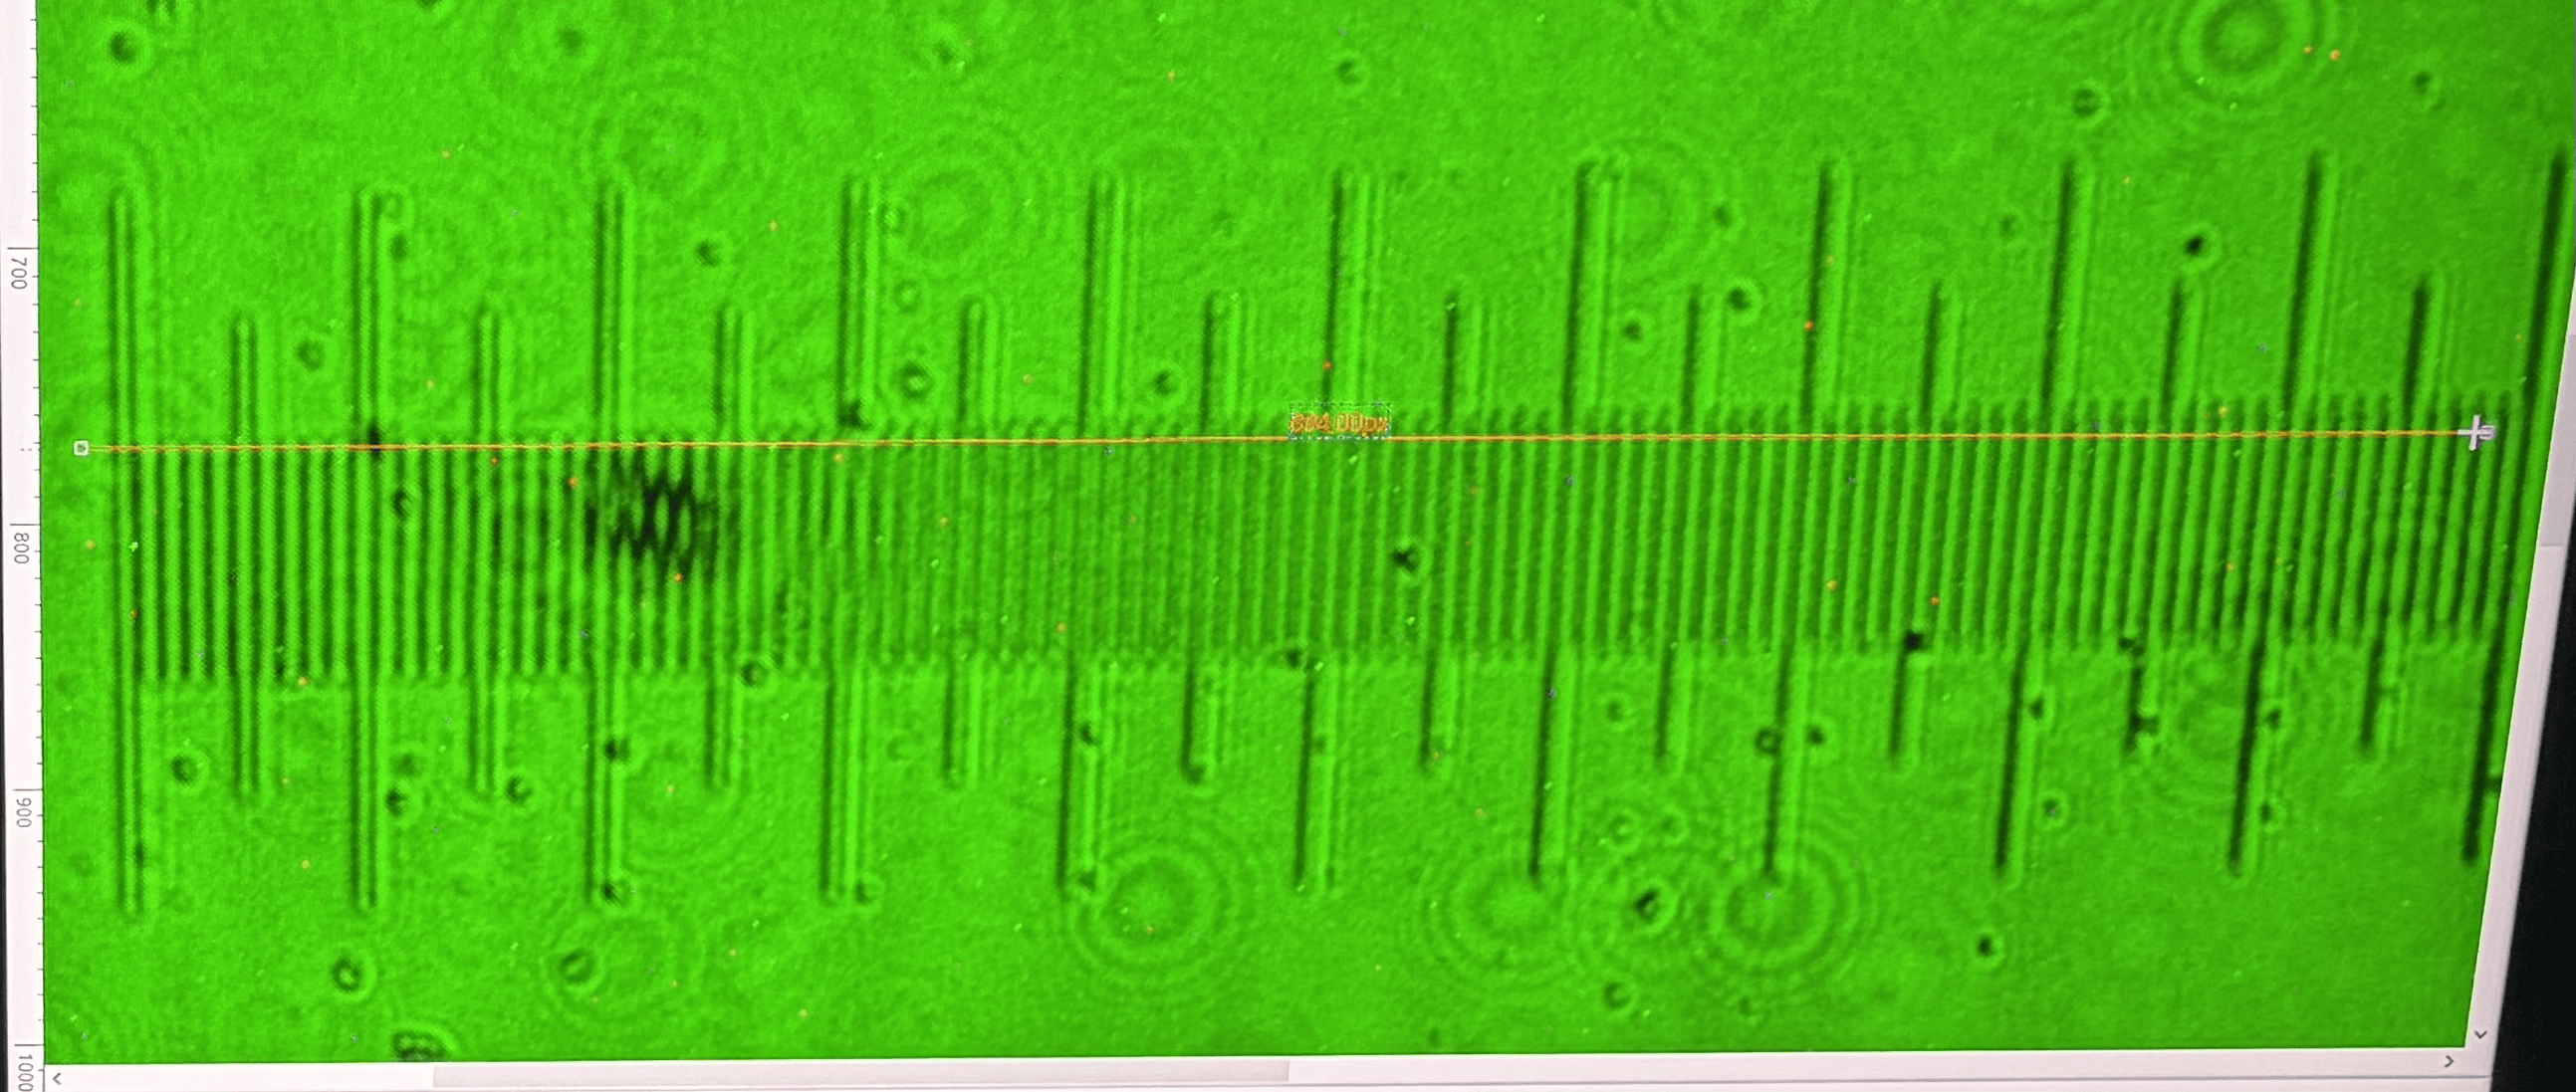
\includegraphics[scale=0.19]{bulk_bullshit.png}}
		\caption{размер 1 мм в пикселях для последующего определения ширины щели $d_2$}
	\end{figure}

Ширина щели в пикселях равна 256 пикселей, тогда ширина в мм будет: $b^\text{pixels} = 256/894 = (0.286 \pm 0.003) $ мм, приняв за $\sigma_b^\text{pixels} = 2 \text{ пикселя} = 0.003 $ мм.

Пронаблюдаем за картиной дифракции при уменьшении $d_2$.
При уменьшении ширины щели уменьшается число зон Френеля, участвующих в формировании дифракционной картины. Вследствие этого изменяется интерференция вкладов от различных участков волнового фронта, нарушается их взаимная компенсация, возрастает роль краёв щели. Щель начинает вести себя как источник с сильной дифракцией. Это приводит к расширению дифракционной картины, изменению распределения интенсивности и уменьшению контраста полос, они становятся более частыми. 



\subsection{Дифракция Фраунгофера на щели}

\begin{figure}[H] 
    \center{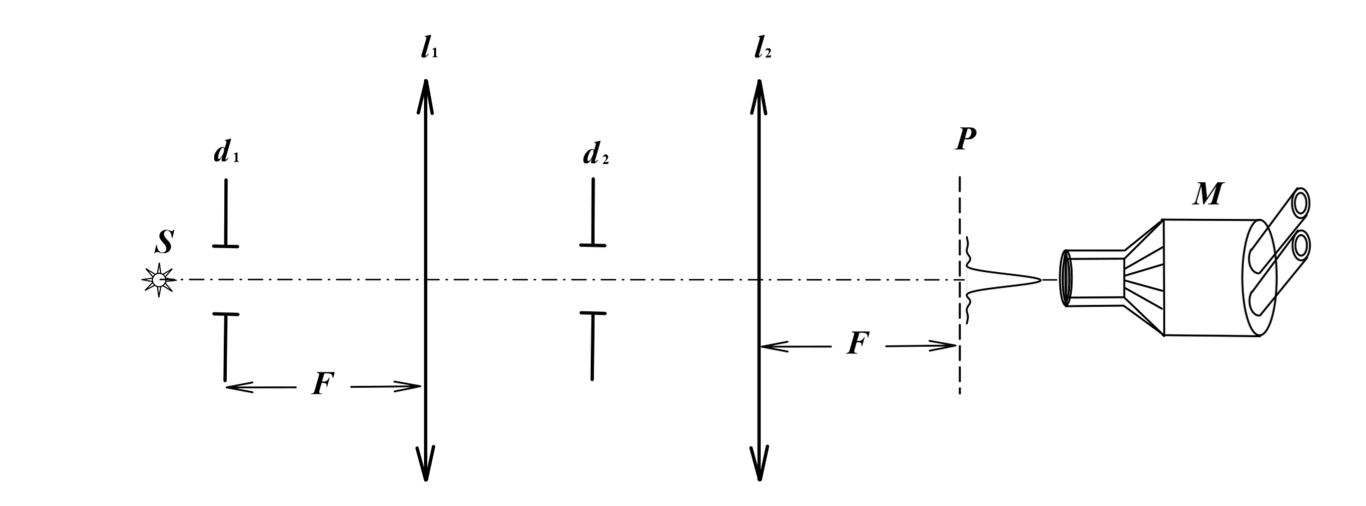
\includegraphics[scale=0.49]{yaustal.png}}
    \caption{Схема установки для наблюдения дифракции Фраунгофера на щели}
\end{figure}

Для наблюдения дифракции Фраунгофера соберем оптическую схему согласно рис. 13. Положения источника света $S$, щели $d_1$ и линзы $l_1$ оставим прежними. Подберем ширину $d_2$ так, чтобы в поле зрения
микроскопа появилась дифракционная картина. В отличие от френелевой дифракционной
картины, фраунгоферова занимает всё поле зрения микроскопа. 


Определим величину ширины щели по микрометрическому винту: $ b = (0.28\pm0.01)$ мм. Фокусное расстояние линзы $ f_2 = 36$ см.

Измерим с помощью измерительных инструментов  видеоокуляра микроскопа координаты $ x_m $ нескольких дифракционных минимумов.  Результаты занесём в Таблицу 2 и построим график зависимости минимумов от их номеров:
из пикселей в мм будем переводить тем, же методом, что выше - знаем, что 1 мм = 894 пикселя и пересчитываем соответственно. Определим погрешность измерений в пикселях: рассмотрим центр интерфереционного минимума и определим размер области, в которой еще можно считать положение центром: $\Delta(X) = 14 \text{ пикселей} = 0.015\text{ мм} $. Определим размер области для дифракционных минимумов, в которой еще можно считать положение центром: $\Delta X_m = 13 \text{ пикселей} = 0.014 \text{ мм}$. Тогда получим, что $\Delta x_m = \sqrt{0.014^2 + 0.015^2} = 0.02 \text{ мм}$.

\begin{table}[H]
\centering
\begin{tabular}{|c|c|c|}
\hline
m & $pixels$ & $x_m, \text{мм}$ \\
\hline
1 & 64 & 0.07 \\
\hline
2 & 116 & 0.13 \\
\hline
3 & 179 & 0.20 \\
\hline
4 & 238 & 0.27 \\
\hline
5 & 295 & 0.33 \\
\hline
6 & 354 & 0.40 \\
\hline
7 & 404 & 0.45 \\
\hline
8 & 465 & 0.52 \\
\hline
\end{tabular}
\caption{Зависимость координат $x_m$ дифракционных минимумов от их номера $ m $}
\end{table}


\begin{figure}[H]
		\center{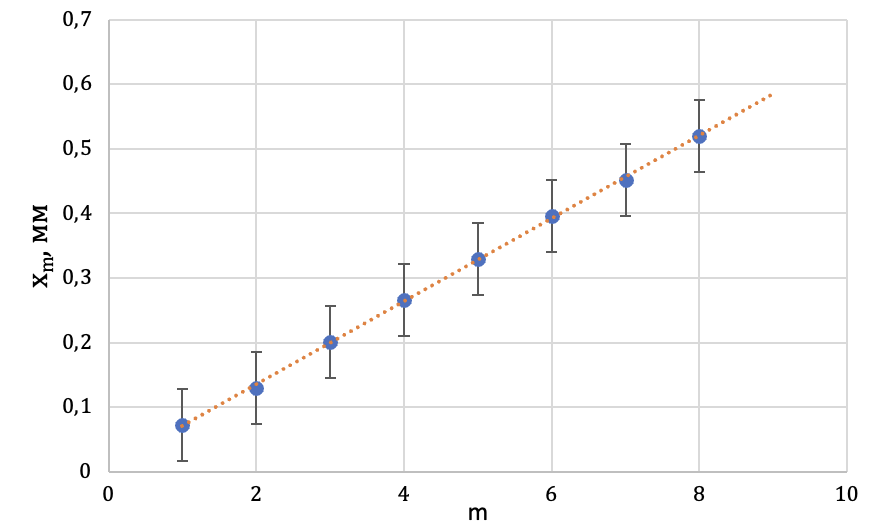
\includegraphics[scale=0.73]{pose_bullshit.png}}
		\caption{график зависимости $x_m(m)$}
	\end{figure}
Определим коэффицент наклона прямой и погрешность по методу наименьших квадратов: 
$$k = (0.064 \pm 0.002) $$

С учетом коэффицента Стьюдента: $\nu = N - 2 = 6$, $t_{P,\nu}\, \approx 2.45$. Тогда $\Delta k = 0.005$.
Из формулы (9) и учитывая погрешность измерений $\Delta x_m$ получаем, что 

$$
b =  \dfrac{\lambda}{k} f =  (0.288 \pm 0.033) \; \text{мм}. 
$$

\begin{figure}[H]
		\center{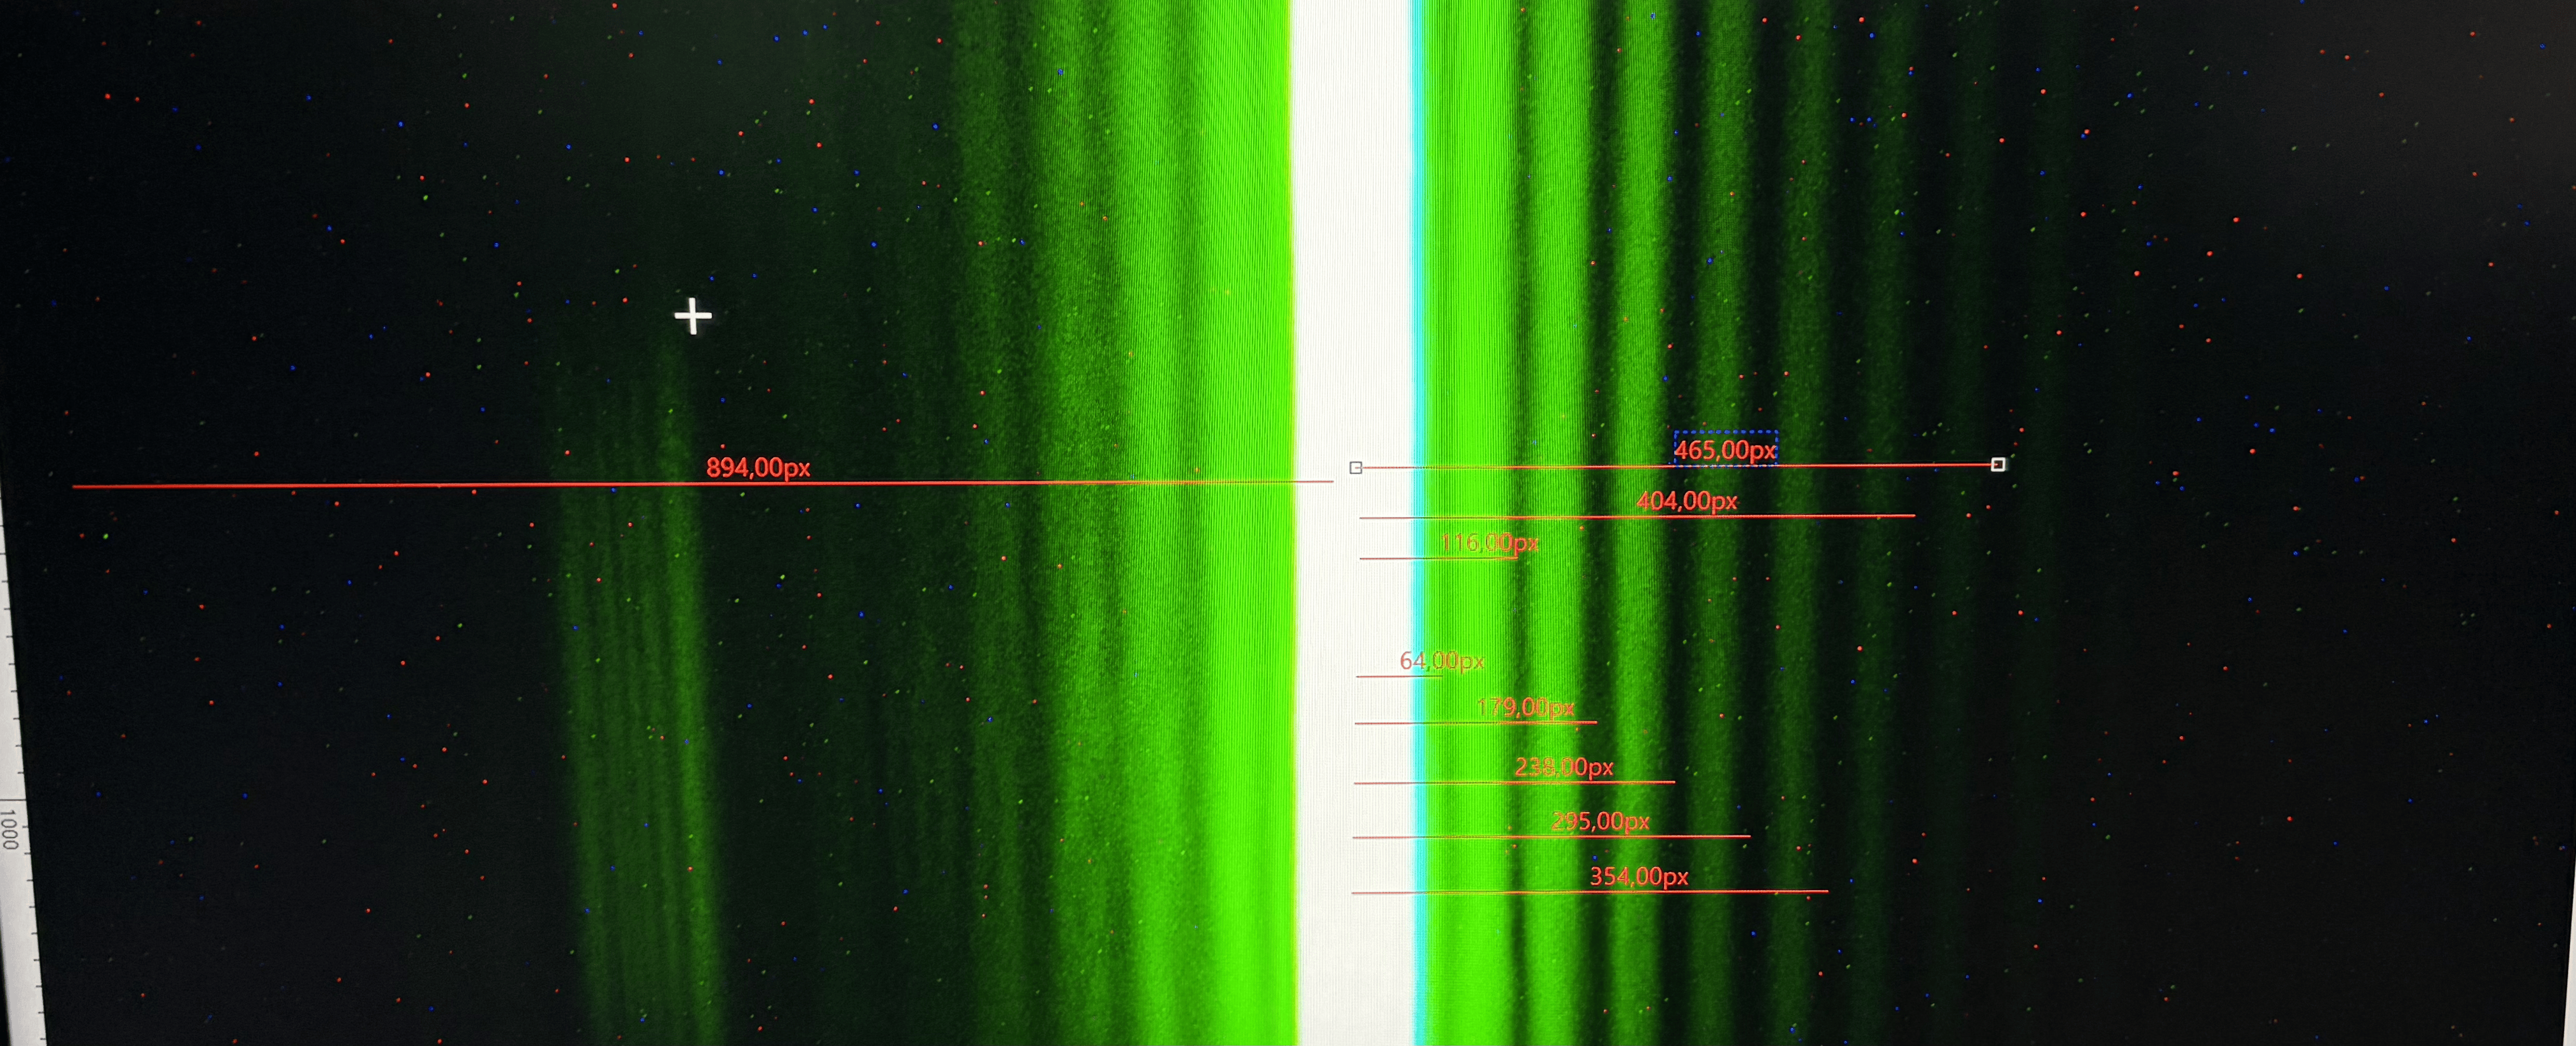
\includegraphics[scale=0.08]{boundary_bullshit.png}}
		\caption{картина дифракции Фраунгофера на одной щели}
	\end{figure}

\subsection{Дифракция Фраунгофера на двух щелях}

\begin{figure}[H]
		\center{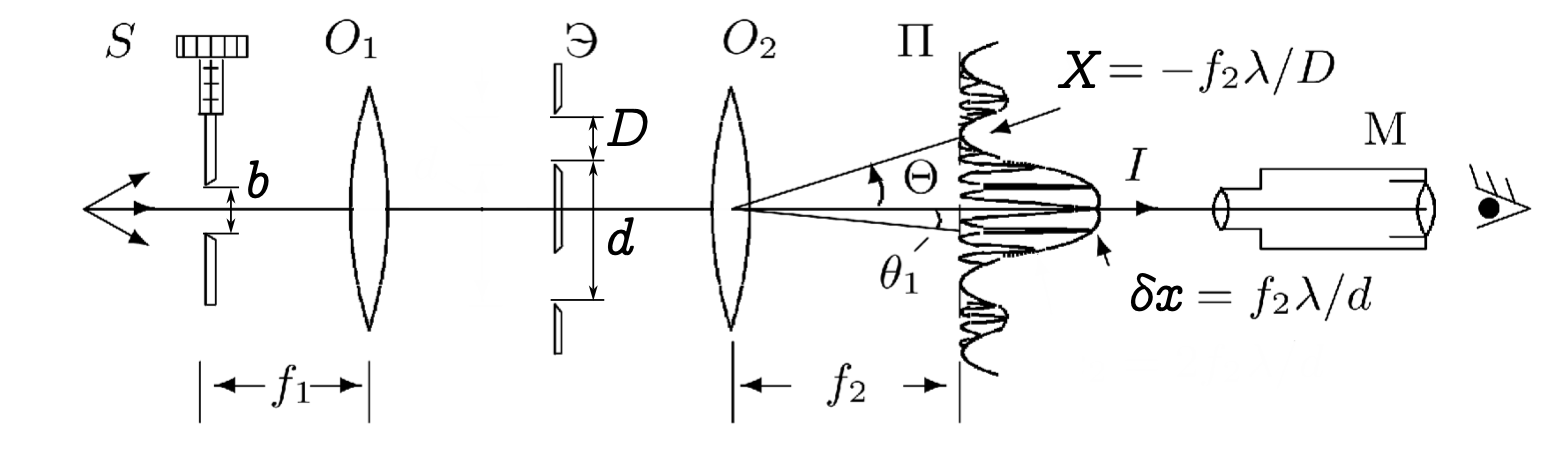
\includegraphics[scale=0.49]{overflow.png}}
		\caption{Схема дифракции Фраунгофера на двух щелях}
	\end{figure}

Результат дифракции на двух щелях можно представить как интерференцию дифракционных картин от каждой щели. 
Поскольку полная угловая ширина главного
дифракционного максимума (от минимума до минимума) равна
$$ \Delta x = 2 \lambda/d, $$
где d — ширина отдельной щели, то на нём укладывается
\begin{equation}
N = 2D/d
\end{equation}
тёмных интерференционных полос (в центре картины максимум, поэтому светлых полос
— на одну больше). Здесь $D$ - расстояние между щелями.
Ширина отдельно взятых интерференционных полос описывается выражением: 
\begin{equation}
    \delta x = f \lambda /D
\end{equation}


Получим на экране дифракционную картину и проведем измерения, результаты занесем в таблицу 3. Для удобства будем сразу пересчитывать расстояние $\delta x$ между минимумами интерференционной картины сразу из пиксели в мм, с учетом, что 1 мм = 894 пикселя. Также определим погрешность измерений в пикселях: рассмотрим центр дифракционного минимума и определим размер области, в которой еще можно считать положение центром, и примем его за погрешность измерения $\Delta(\delta x)$: $\Delta(\delta x) = 12 \text{ пикселей} = 0.01 \text{ мм} $.
\begin{table}[H]
\centering
\begin{tabular}{|l|c|c|c|c|c|c|}
\hline
$\delta x$, pixels & 84 & 86 & 84 & 86 & 87 & 86 \\
\hline
$\delta x$, мм & 0.094 & 0.096 & 0.094 & 0.096 & 0.097 & 0.096    \\
\hline
\end{tabular}
\caption{расстояния $\delta x$ между минимумами интерференционной картины}
\end{table}
Определим число $N$ тёмных интерференционных полос в пределах главного дифракционного максимума: $N = 8$.

% подберите такую ширину входной щели $d_0$,
% при которой наступает первое исчезновение интерференционных полос: 


\begin{figure}[H]
		\center{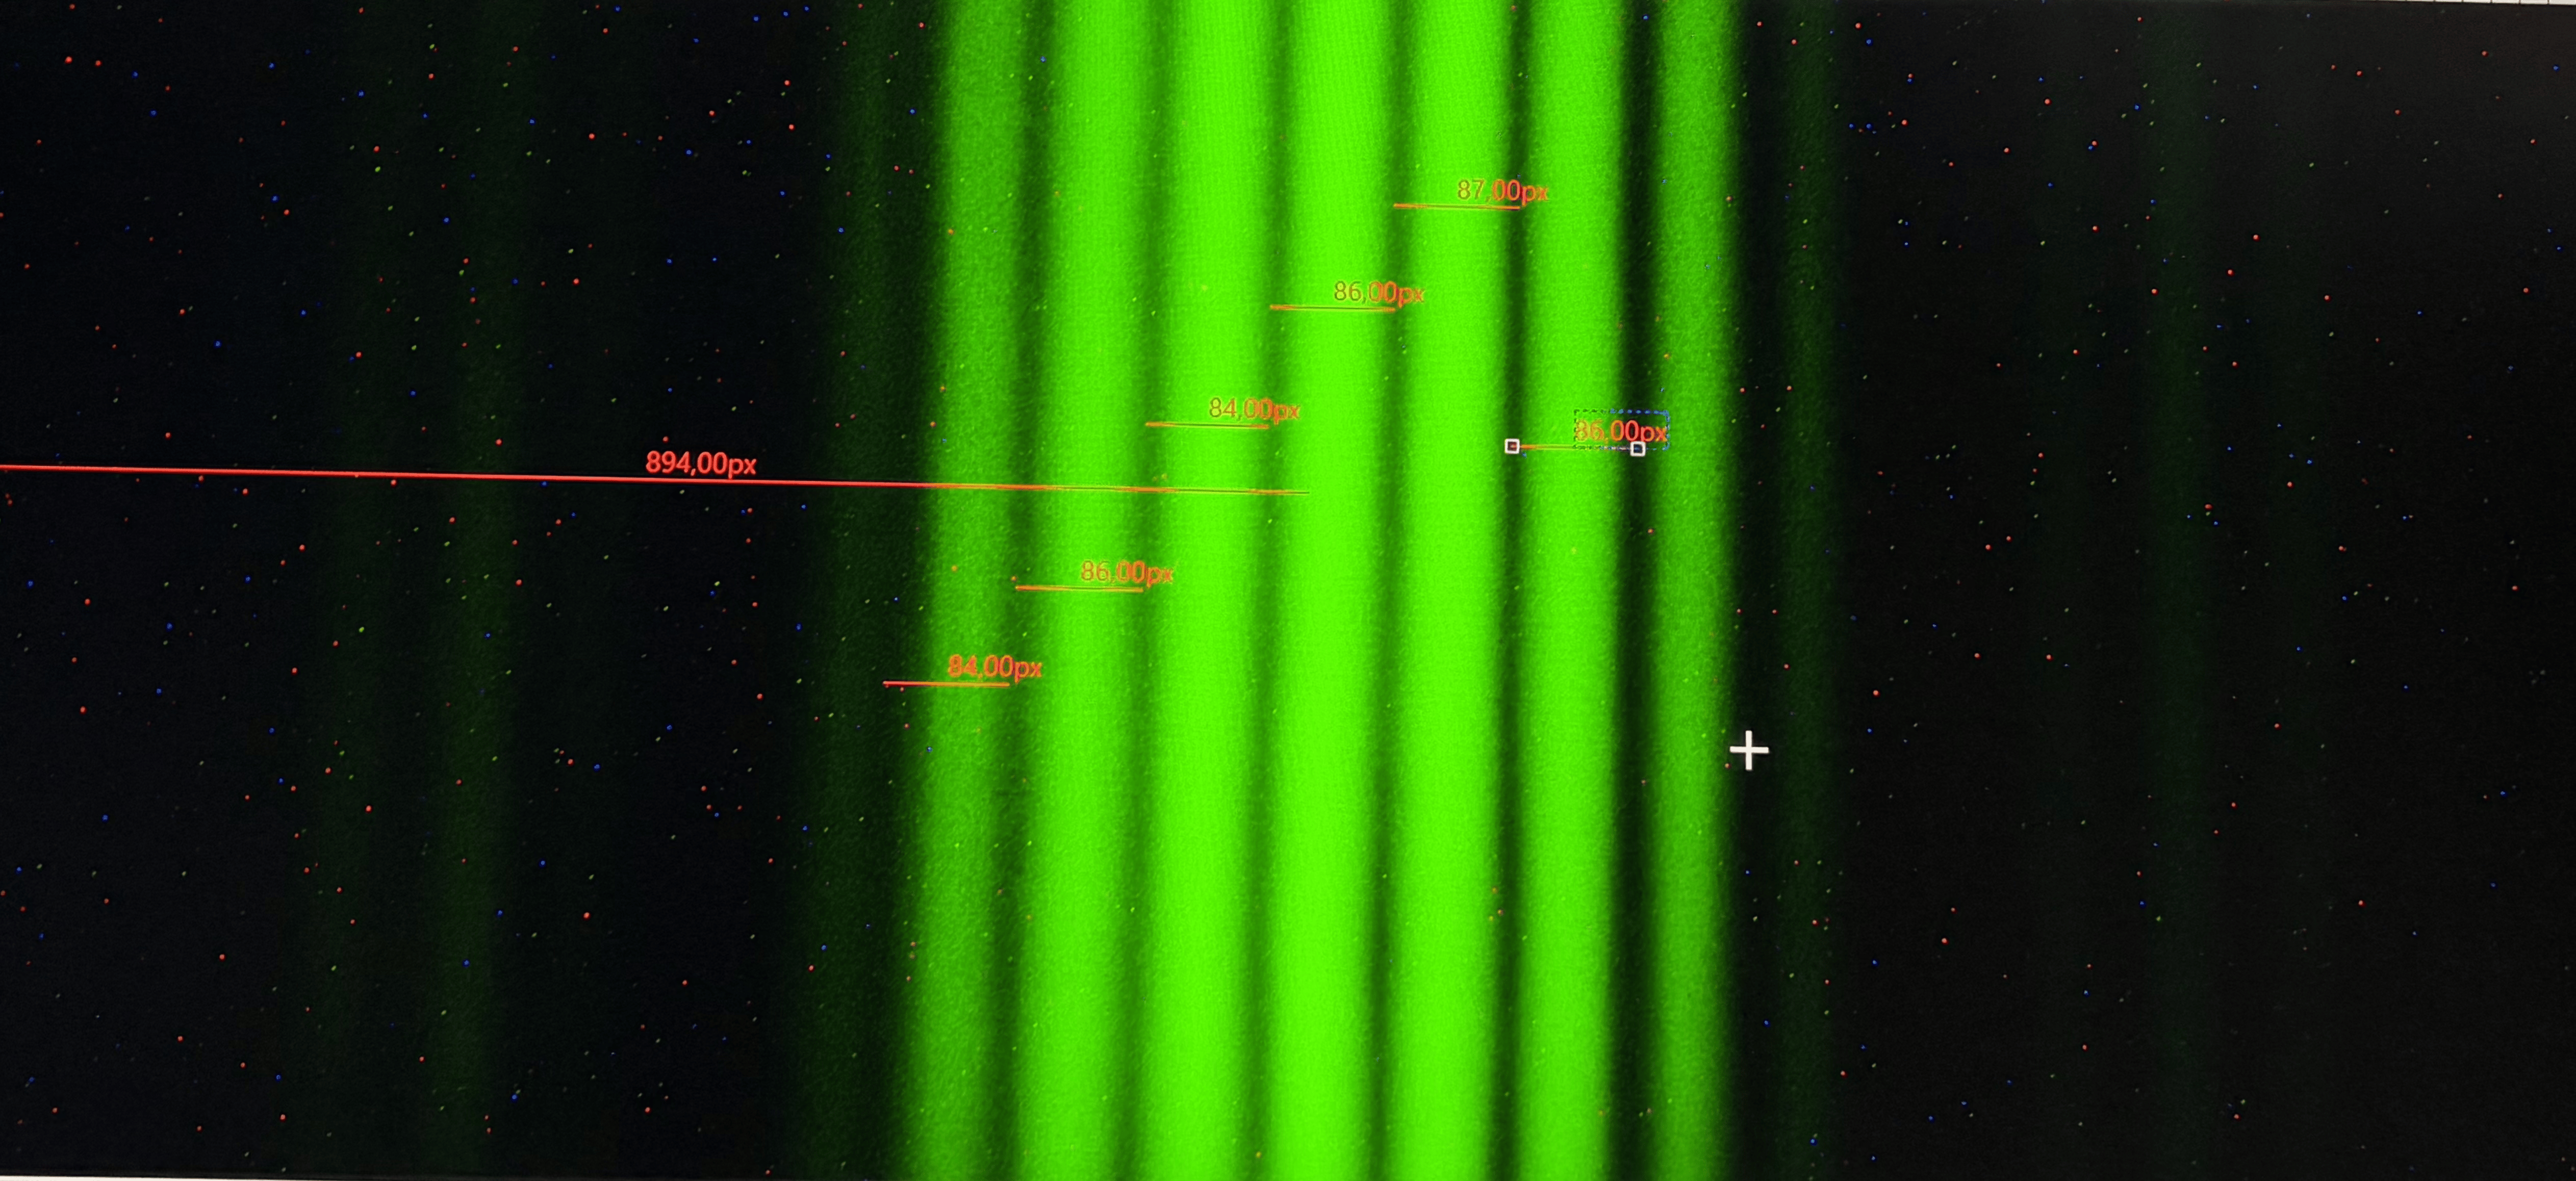
\includegraphics[scale=0.08]{polniy_bullshit.png}}
		\caption{картина дифракции Фраунгофера на двойной щели}
	\end{figure}

 По расстоянию между полосами, рассчитаем по формуле (21) расстояние между щелями: 

$$D^{\text{расч}} = (1.97 \pm 0.03 ) \text{ мм} $$

Определим ширину двойных щелей и расстояние между щелями по фото, с учетом, что диаметр линзы равен 50.8 мм = 640 пикселей: 
$$d^\text{изм} = (0.47 \pm  0.05) \text{ мм} $$
$$D^{\text{изм}} = (1.64 \pm 0.05) \text{ мм} $$

За погрешность я взял 20 пикселей = 0.05 мм.
% , так как точность данного метода невысокая.

 Сравним наблюдаемое число полос в главном максимуме с теоретическим, расчитанным по формуле (20):
 
 $$N^{\text{расч}} = 6.98$$

 $$N^{\text{изм}} = 8$$

Оценим ширину входной щели по формуле (13):

$$d_1 \approx \frac{\lambda f}{D} = (0.113 \pm 0.003) ~\text{ мм} $$ 

Сравним ее с шириной, определенной микрометрическим винтом: 

$$d_1^{\text{винт}} = (0.16 \pm 0.01) ~\text{мм}$$

\subsection{Дифракция Френеля на круглых препятствиях}
Соберем установку согласно оптической схеме на рис. 18:
\begin{figure}[H]
		\center{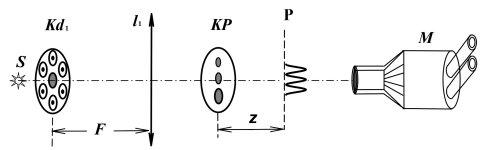
\includegraphics[scale=1.2]{prepyatstviya.png}}
		\caption{}
	\end{figure}

где Kd - барабан с возможностью выбора отверстия, выполняющего роль вторичного источника света, l - линза, KP - пластинка с возможностью выбора круговых препятствий различного размера.

Поместим в поле зрения микроскопа одно из круглых препятствий, и отодвинем микроскоп на такое расстояние, чтобы получить четкое изображение на экране. Убедимся, что при удалении микроскопа от препятствия на изображении всегда появляется светлое пятно.

\begin{figure}[h!]
        \begin{center}
            \begin{minipage}[h!]{0.31\linewidth}
                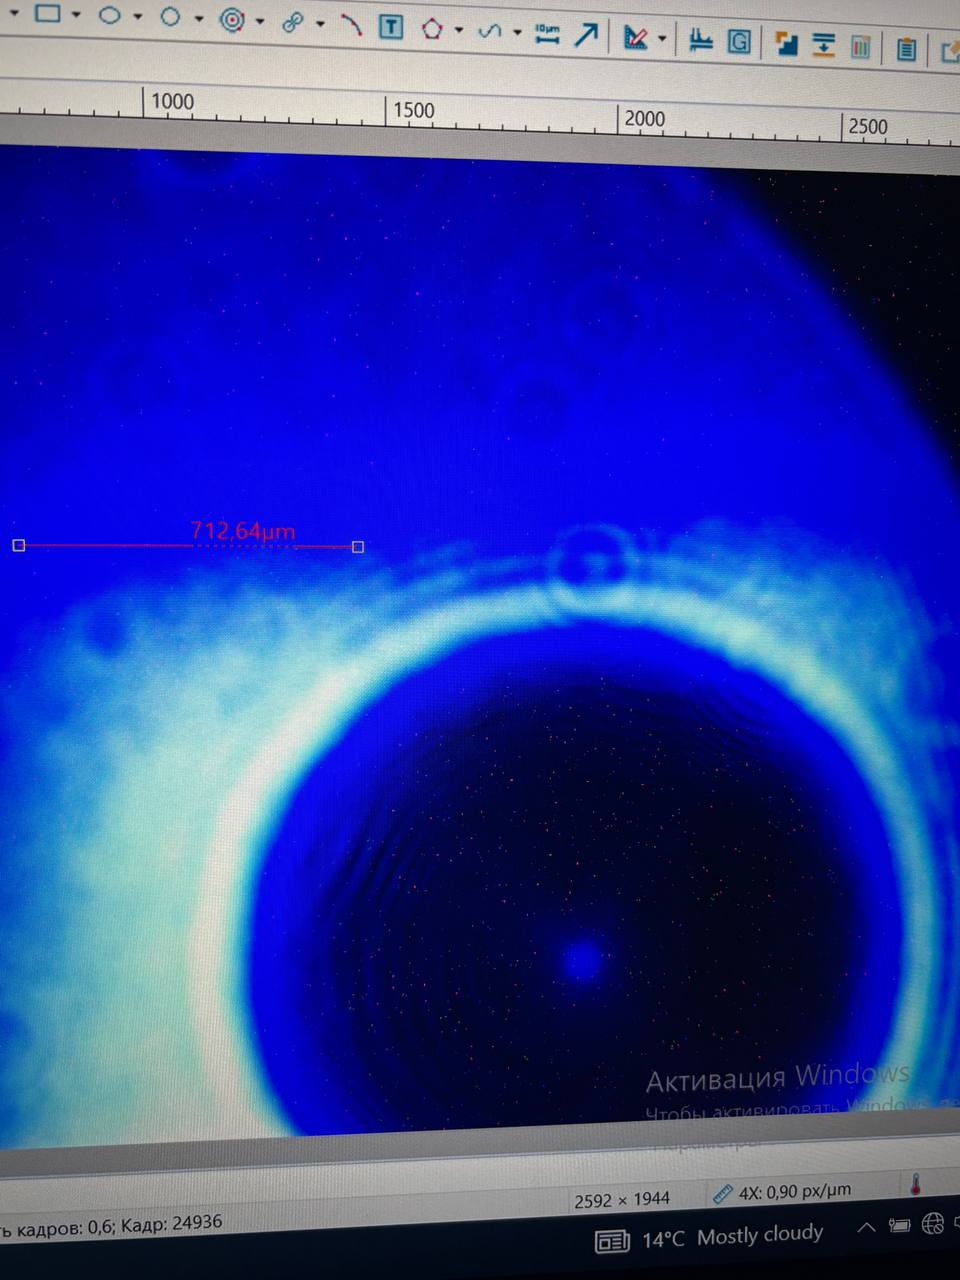
\includegraphics[width=1\linewidth]{vnutr_mal.jpg}
                \caption{Светлое пятно}
                \label{picture_2}
            \end{minipage}
            \hfill
            \begin{minipage}[h!]{0.56\linewidth}
                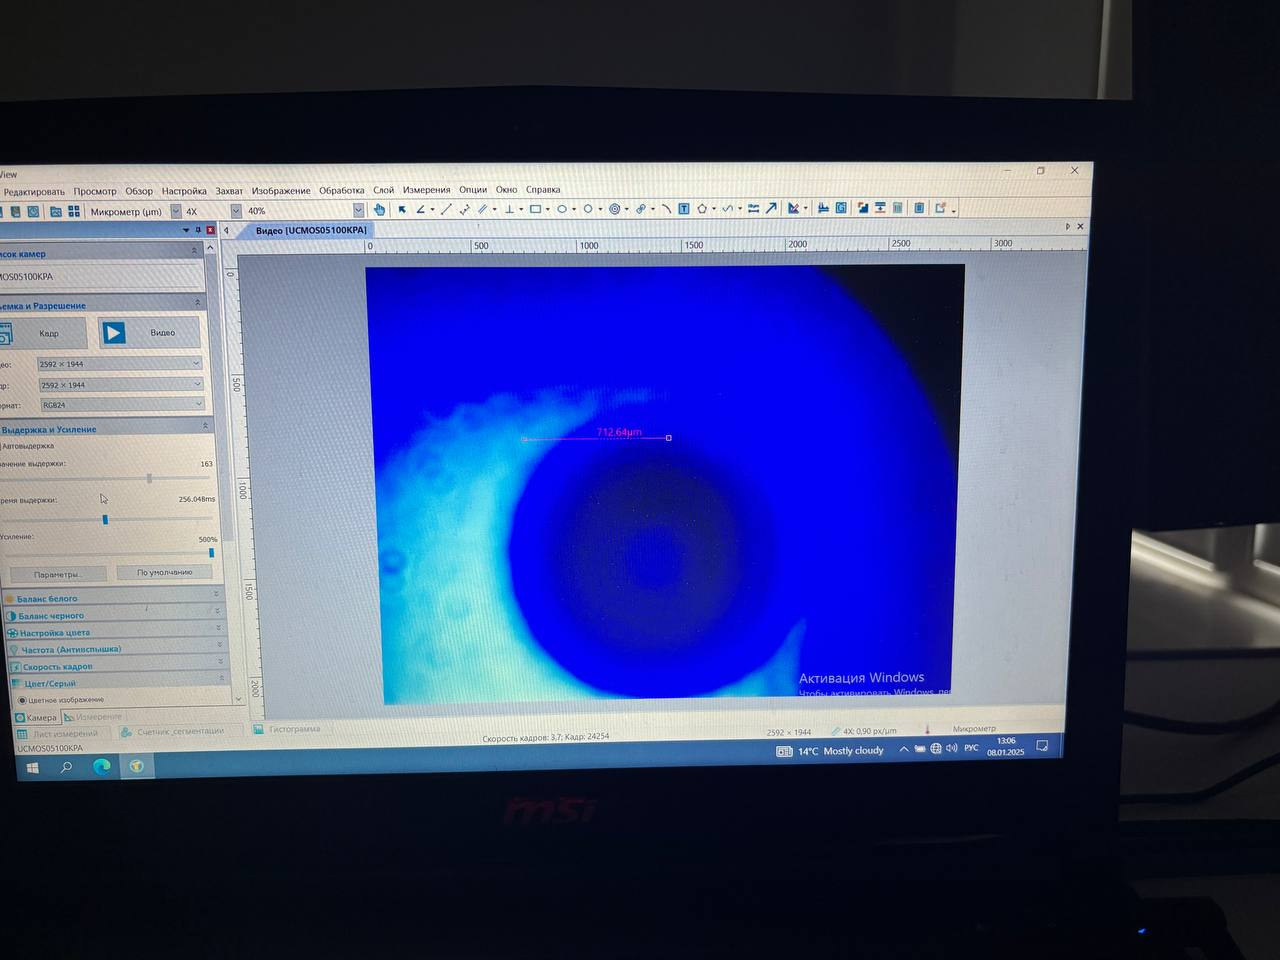
\includegraphics[width=1\linewidth]{vnutr.jpg}
                \caption{Светлое пятно при другом препятствии}
                \label{picture_3}
            \end{minipage}
        \end{center}
    \end{figure}

\subsection{Дифракция Френеля на круглых отверстиях}
Соберем установку согласно оптической схеме на рис. 21:
\begin{figure}[H]
		\center{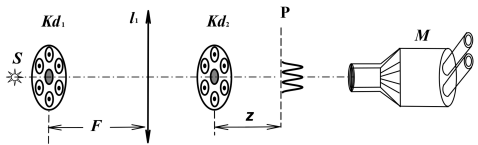
\includegraphics[scale=1.2]{otverstiya.png}}
		\caption{}
	\end{figure}

где Kd1 - барабан с возможностью выбора отверстия, выполняющего роль вторичного источника света, l - линза, Kd2 - пластинка с возможностью выбора круговых отверстий различного размера, утановленная максимально близко к линзе.

Перемещая микроскоп вдоль оптической оси, установим его таким образом,
чтобы было видно резкое изображение отверстия в кассете Kd2. 

Пронаблюдаем, как при удалении микроскопа появляются узкие тёмные дифракционные кольца, количество которых уменьшается по мере удаления микроскопа

\begin{figure}[H]
		\center{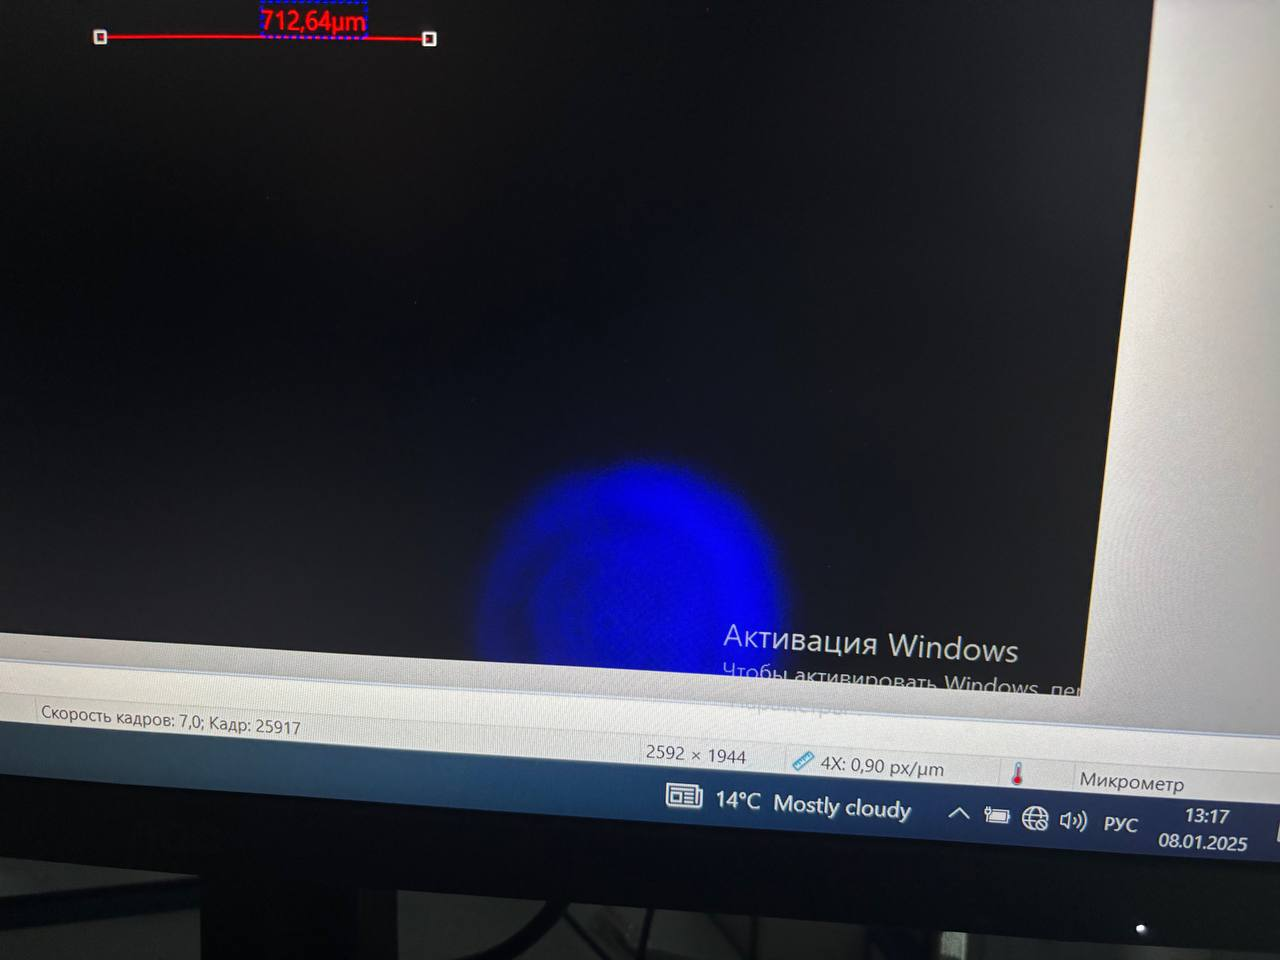
\includegraphics[scale=0.35]{naruzh.jpg}}
		\caption{Дифракция Френеля на отверстии с темными кольцами}
	\end{figure}


\newpage
\section{Заключение. Обсуждение и выводы}
Была проведена работа, целью которой являлось исследование явлений дифракции Френеля на щели, дифракции Фраунгофера на одной и двух щелях, а также дифрации Френеля на круглых препятствиях и отверстиях. Вначале была исследована дифракция Френеля на щели: была получена линейная зависимость координаты микроскопа $z$ от числа $ n $ тёмных полос, которая хорошо аппроксимировалась прямой. По микрометрическому винту и по данной зависимости была определена ширина щели $d_2$:

$$ b^\text{винт}_{\text{френель}} = (0.30 \pm 0.01)  \text{ мм; } ~ b^{\text{расч}}_\text{френель}  = (0.27 \pm 0.06) ~\text{мм}$$ Как видим, значения достаточно близки, относительные погрешности же отличаются: 
$$\varepsilon_{b^\text{винт}_\text{френель}} = 3.3 \% ; ~\varepsilon_{b^{\text{расч}}_\text{френель}} = 22.2 \% $$

Далее была исследована дифракция Фраунгофера на одной щели:
Также по микрометрическому винту и по зависимости координат $x_m$ дифракционных минимумов от их номера $ m $ была определена ширина щели $d_2$:

$$ b^\text{винт}_\text{фр1} = (0.28 \pm 0.01)  \text{ мм; } ~ b^{\text{расч}}_\text{фр1}  = (0.288 \pm 0.033) ~\text{мм}$$ Опять же, как видим, значения достаточно близки:
$$\varepsilon_{b^\text{винт}_\text{фр1}} = 3.7 \% ; ~\varepsilon_{b^{\text{расч}}_\text{фр1}} = 11.5 \% $$


Была исследована дифракция Фраунгофера на двойной щели. Было определено число $N$ тёмных интерференционных полос в пределах главного дифракционного максимума: $N = 8$. Видно, что оно отличается от расчитанного: $N^{\text{расч}} = 6.98$. Также и отличаются расстояния между щелями $D^{\text{расч}} = (1.97 \pm 0.02 ) \text{ мм} $ и $D^{\text{изм}} = (1.64 \pm 0.05) \text{ мм} $, и ширина входной щели: $d_1^{\text{винт}} = (0.16 \pm 0.01) ~\text{мм}$ и $d_1 = (0.113 \pm 0.003) ~\text{ мм} $. Это может быть связано с неточностью определения ширины двойных щелей и расстояния между щелями по фото, так как это не самый точный метод. Несмотря на это, относительные погрешности достаточно низки: $$\varepsilon_{D^{\text{расч}}} = 1.5\%, \quad 
\varepsilon_{D^{\text{изм}}} = 3.0\%, \quad 
\varepsilon_{d_1^{\text{винт}}} = 6.3\%, \quad 
\varepsilon_{d_1} = 2.7\% $$

Продемонстрирована дифракция Френеля на круглых препятствиях и отверстиях. В случае препятствий на изображении присутствовало светлое пятно в темном круге, сохраняющееся при удалении микроскопа. В эксперименте с отверстиями на изображении появляются узкие темные дифракционные кольца (сначала у краев), количество которых уменьшается при удалении микроскопа.

\end{document}
